% !TEX root = ../patchEmbeddings_review.tex

\begin{figure}[t]
\centering
        % \includegraphics[width=0.4\textwidth,trim=0.25in 0.25in 0.68in 0.36in,clip]{./figs/SSBM_experiments.pdf} % 0.45
        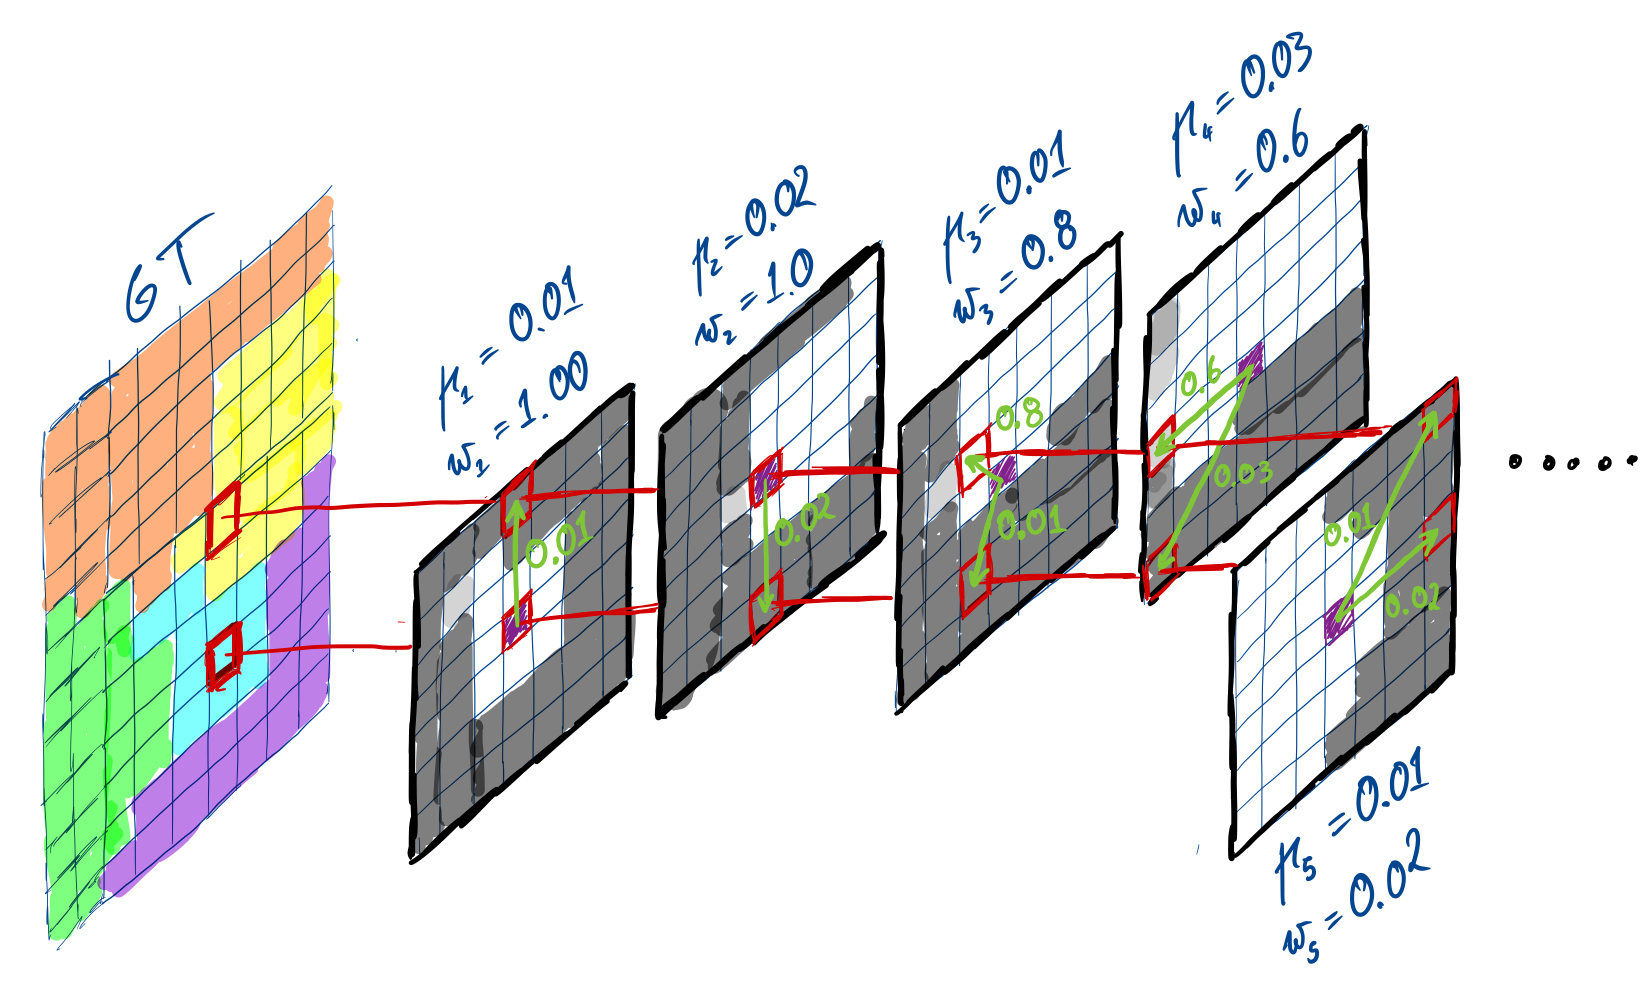
\includegraphics[width=0.7\textwidth]{./figs/alg_explaned.jpg} % 0.45
        \caption{Illustration of the proposed parameter-free method to convert self-probability masks to edge weights...}
    \label{fig:alg_explained}
\end{figure}
\begin{algorithm}[t]
  \begin{flushleft}
  \caption{: Computing affinities from self-probability masks}
   \hspace*{\algorithmicindent} \textbf{Input:} Graph $\mathcal{G}(V,E)$; local self-probability masks $\mathcal{M}_{\mathbf{x}}: \mathcal{N}_{K\times K} \rightarrow [0,1]$  \\
  \hspace*{\algorithmicindent} \textbf{Output:} Affinities $\bar{a}_e\in[0,1]$ with variance $\sigma^2_e$ for all edges $e\in E$\\
  \hspace*{\algorithmicindent} 
  \begin{algorithmic}[1]
  \footnotesize
  % \small
      % \State Initial clustering: $\Pi=\{\{v_1\}, \ldots, \{v_{|V|}\}\}$
      % \State Initialize interactions between clusters with $ = w^+_e - w^-_e$
      \For{each edge $e\in E$ in graph $\mathcal{G}$}
        \State Get coordinates $\mathbf{x}=(x_1,x_2)$ and $\mathbf{y}=(y_1,y_2)$ of pixels linked by edge $e$
        \State Init. accumulation sets $\mathcal{A}=\{\}$ for affinities and $\mathcal{W}=\{\}$ for reliability weights
        \For{each mask $\mathcal{M}_{\mathbf{c}}$ covering both pixel $\mathbf{x}$ and pixel $\mathbf{y}$}
            \State Get relative coords. $\delta_\mathbf{x}$ and $\delta_\mathbf{y}$ with respect to the center $\mathbf{c}$ of the mask $\mathcal{M}_{\mathbf{c}}$
            \State $\mathcal{A}\,\gets \mathcal{A} \,\cup\,\{\min \big(\mathcal{M}_{\mathbf{c}}(\delta_\mathbf{x}), \,\mathcal{M}_{\mathbf{c}}(\delta_\mathbf{y})\big)\}$ \Comment{Fuzzy-AND: both values active}
            \State $\mathcal{W}\gets \mathcal{W} \,\cup\,\{\max \big(\mathcal{M}_{\mathbf{c}}(\delta_\mathbf{x}), \,\mathcal{M}_{\mathbf{c}}(\delta_\mathbf{y})\big)\}$ \Comment{Fuzzy-OR: at least one value active}
        \EndFor
        \State Get weighted average $\bar{a}_e= (\sum_{a\in\mathcal{A}}\sum_{w\in\mathcal{W}} \,w\cdot a)\,/\,(\sum_{w\in\mathcal{W}}\,w)$ 
        \State Get weighted variance $\sigma^2_e = \big(\sum_{a\in\mathcal{A}}\sum_{w\in\mathcal{W}} \,w\cdot (a-\bar{a}_e)^2\big)\,/\,\big(\sum_{w\in\mathcal{W}}\,w\big)$
      \EndFor
      \State
      \Return $a_e, \sigma^2_e$ for each $e\in E$
  \end{algorithmic}
    \label{computing_affinities}
  \end{flushleft}

\end{algorithm}

\section{Computing affinities from self-probability masks}
\TODO{To be completed}
% A lot of recently proposed instance-segmentation methods, predict pairwise affinity between pairs of pixels 
By predicting a self-probability mask for each pixel, the pairwise affinity between two pixels is predicted 


One common used method is to predict a set of sparse affinities for every pixel (see Fig. \ref{fig:comparing_masks_affs}c)... 
These can then be see as edge weights of a grid-graph where each node represents a pixel of the image. And a graph clustering algorithm is then applied to output an instance segmentation.
In this section, we propose to ways to perform something similar and use the predicted per-pixel self-probability masks to define the edge weights of a grid-graph.
First, in Sec. \ref{sec:efficient_affs} we propose a simple way to efficiently extract a set of sparse affinities from the predicted encoded self-probability masks, without the need to decode them one by one. Then, in Sec. \ref{sec:prob_affs}...

\subsection{Efficient computation of sparse affinities from encoded masks}\label{sec:efficient_affs}
A commonly used instance segmentation method predicts, for each pixel, a small set of sparse short- and long-range affinities representing how likely it is for a pair of pixels to belong to the same object instance (see Fig. \ref{fig:comparing_masks_affs}c).



As a second contribution, we propose two distinct ways of converting the predicted per-pixel self-probability masks into edge weights of a graph representing the image, so that each node corresponds to a pixel and a graph clustering algorithm is then used to output an instance segmentation.

Here it would be nice to claim that hopefully the set of affinities we get out of this leads to more consistent neighborhood structures as compared to directly predicting each affinity as an output channel of the main model

\subsection{Averaged }\label{sec:prob_affs}
\begin{itemize}
\item Every patch predicts $M\times N$ affinities between the central pixel and the neighboring ones. But can we do better?
\item Defining the graph: we have an edge between two nodes $(i, j)$ only if $j \in M\times N$ Given two pixels  
\end{itemize}
- 


The second proposed method yields a parameter-free algorithm achieving competitive performances, yada yada yada... 



